\documentclass[11pt]{article}
\usepackage{graphicx}
\usepackage{subcaption}
\usepackage[table]{xcolor}
\usepackage{float}
\usepackage[a4paper,margin=2cm]{geometry}
\usepackage{fancyhdr}
\usepackage{listings}

\lstnewenvironment{rc}[1][]{\lstset{language=R}}{}
\newcommand{\ri}[1]{\lstinline{#1}}  %% Short for 'R inline'

\lstset{language=R}             % Set R to default language

\begin{document}

\title{STAT 565 HW-3}
\author{Yokesh Thirumoorthi}

\maketitle
\pagestyle{fancy}
\fancyhf{}
\rhead{Yokesh Thirumoorthi}
\lhead{STAT 565 HW-3 Winter 2020}
\rfoot{Page \thepage}

\section{Question 1}

In this problem I need to compare $\displaystyle a=3$ treatments (brochure design), 
but the data is being influenced by $\displaystyle b=4$ blocks (regions).

% Each datapoint can be thought of as the sum of several factors,
% $$\displaystyle y_{ij}=\mu +\tau _{i}+\beta _{j}+\epsilon _{ij}$$

% Where:

% $\displaystyle i=1,2,...,a$

% $\displaystyle j=1,2,...,b$

% and:
% $\displaystyle y_{ij}=$ datapoint from the $\displaystyle i$th treatment and the $\displaystyle j$th block

% $\displaystyle \mu =$ the grand mean

% $\displaystyle \tau _{i}=$ the effect of the $\displaystyle i$th treatment

% $\displaystyle \beta _{j}=$ the effect of the j $\displaystyle j$th block

% $\displaystyle \epsilon _{ij}=$ a random error affecting the datapoint from the $\displaystyle i$th treatment and the $\displaystyle j$th block

% $\linebreak$

Analyse the data using ANOVA table, which is generated using below R code

\begin{lstlisting}[language=R]
    Design <- factor( rep(c(1,2,3), each=4) )
    Region <- factor( rep(c("NE", "NW", "SE", "SW"), 3))
    Mail  <- c(250, 350, 219, 375, 
                400, 525, 390, 580, 
                275, 340, 200, 310)
    options(contrasts=c("contr.treatment","contr.poly"))
    model=lm(Mail~Region+Design)
    summary(aov(model))    
\end{lstlisting}

\lstinputlisting[float=h,frame=tb,caption=R output,label=zebra]{../out/hw3_q1_anova.txt}

The model F-value of 50.15 implies the model is significant.

\paragraph{}
Fisher LSD comparisons allow each pair of treatment means to be compared. 

If $\displaystyle \mid \bar{y_i} - \bar{y_j} \mid > LSD$ then the treatment means  $\displaystyle i$ and $\displaystyle j$ are significantly different. 

Determine the treatment means using below R code

\begin{lstlisting}[language=R]
    mean(Mail[Design == 1])
    mean(Mail[Design == 2])
    mean(Mail[Design == 3])  
    
    library(agricolae)
    LSD.test(model,"Mail")
\end{lstlisting}

\lstinputlisting[float=h,frame=tb,caption=R output,label=zebra]{../out/hw3_q1_means.txt}

Thus we have the treatment means as,
$\displaystyle \mu_1=298.5, \mu_2=473.75, \mu_3=281.25$

Based on examination of the plot, we would conclude that 
$\displaystyle \mu_1$ and $\displaystyle \mu_3$ are the same.
$\displaystyle \mu_2$ differs from $\displaystyle \mu_1$ and $\displaystyle \mu_3$;

\subsection{Residual Analyses}

\begin{figure}[H]
    \centering
    \begin{subfigure}{0.45\textwidth}
        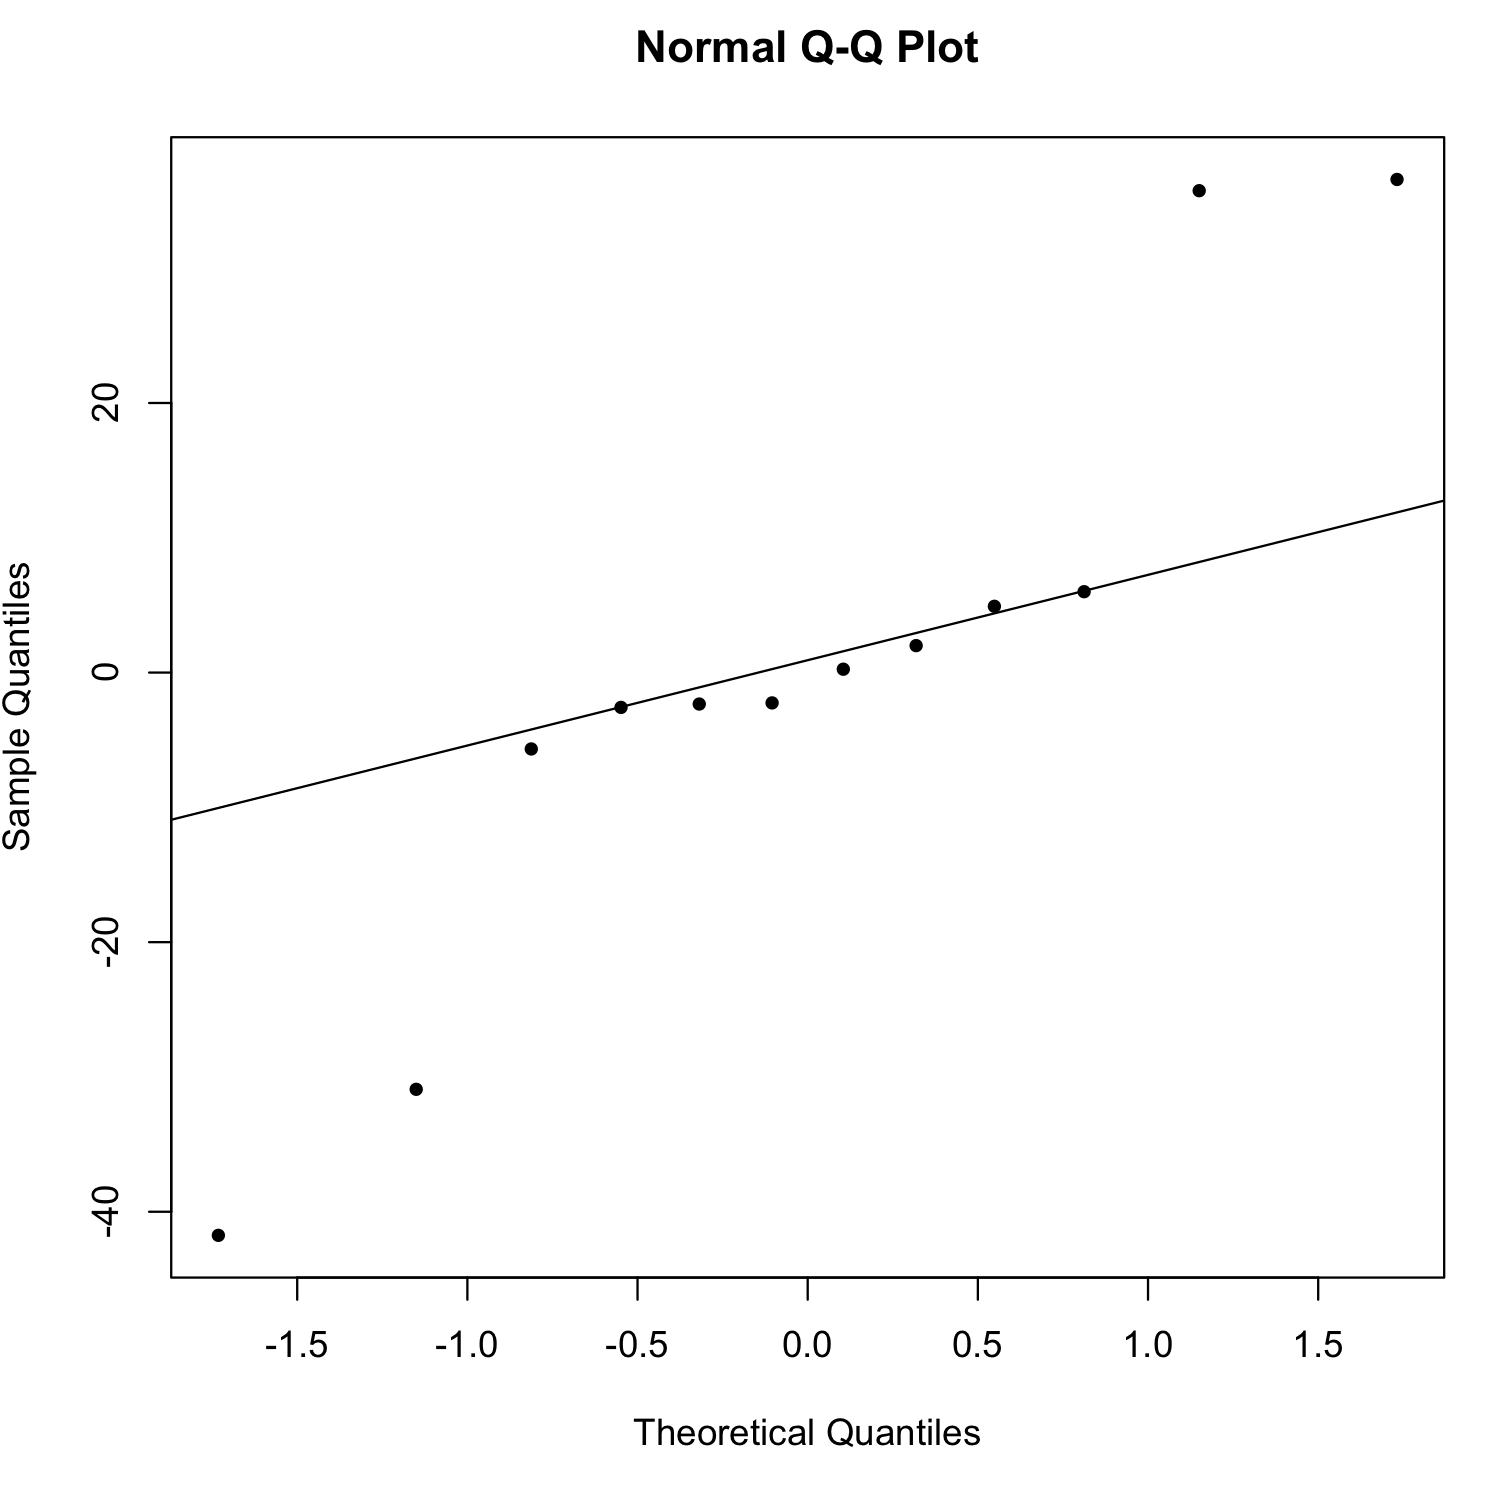
\includegraphics[width=\textwidth]{../pictures/hw3_q1_1_qq.png}
    \end{subfigure}
    \begin{subfigure}{0.45\textwidth}
        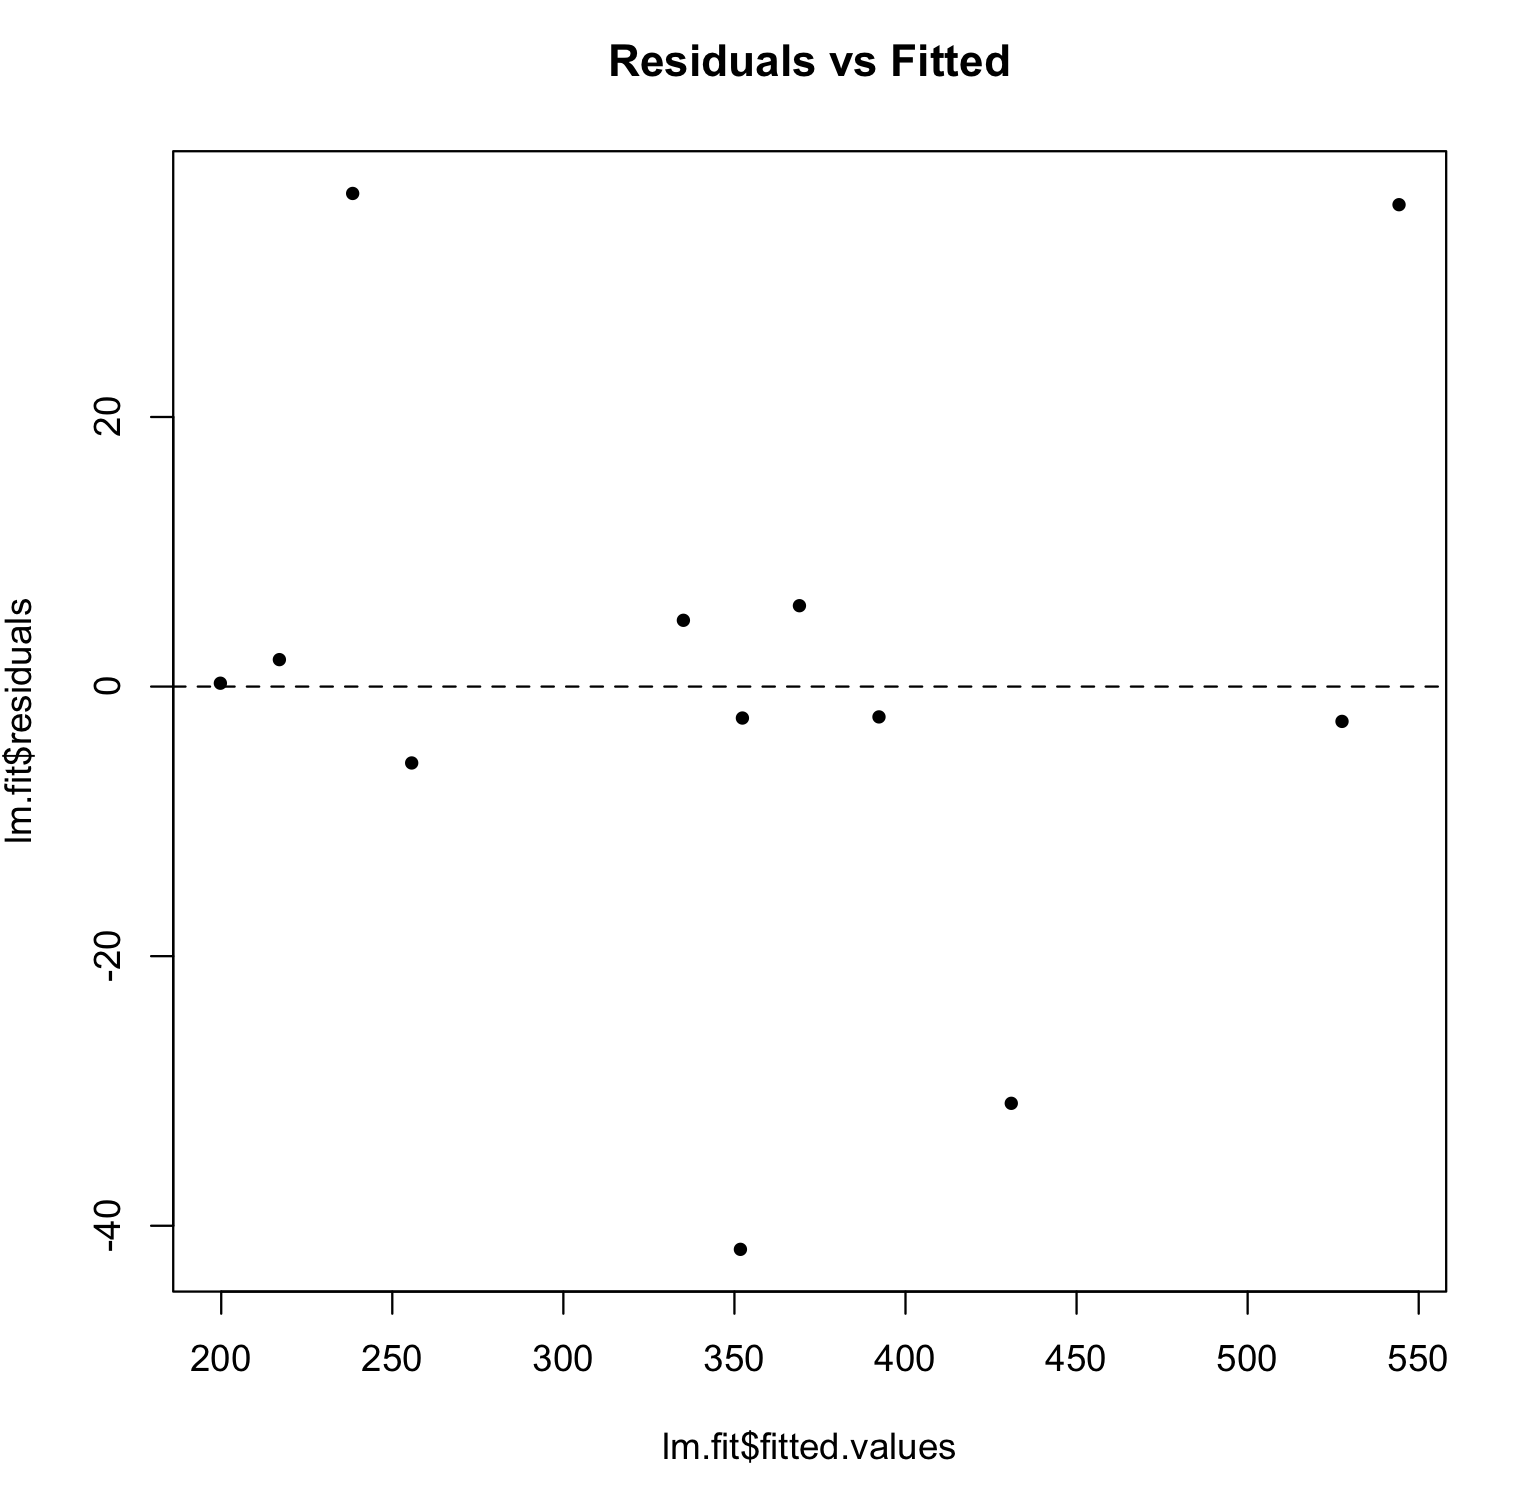
\includegraphics[width=\textwidth]{../pictures/hw3_q1_1_nf.png}
    \end{subfigure}
\end{figure}

There seem to be a problem with normality as the plots are generally not in a straight line.
And the residuals are not equally distributed around the 0 and shows inequality of variance.

\section{Question 1 - Data Transformation}
Since the residuals of the model generated by fitting the given data are not normally distributed,
I applied a square root transformation. The ANOVA table is generated using below R code,

\begin{lstlisting}[language=R]
    
    T_sqrt = sqrt(Mail)
    plotNormalHistogram(T_sqrt)

    t_model=lm(T_sqrt~Region+Design)
    summary(aov(t_model))
  
\end{lstlisting}

\lstinputlisting[float=h,frame=tb,caption=R output,label=zebra]{../out/hw3_q1_2_anova.txt}

The model F-value of 60.47 implies the model is significant.


\subsection{Residual Analyses on transformed data}

\begin{figure}[H]
    \centering
    \begin{subfigure}{0.45\textwidth}
        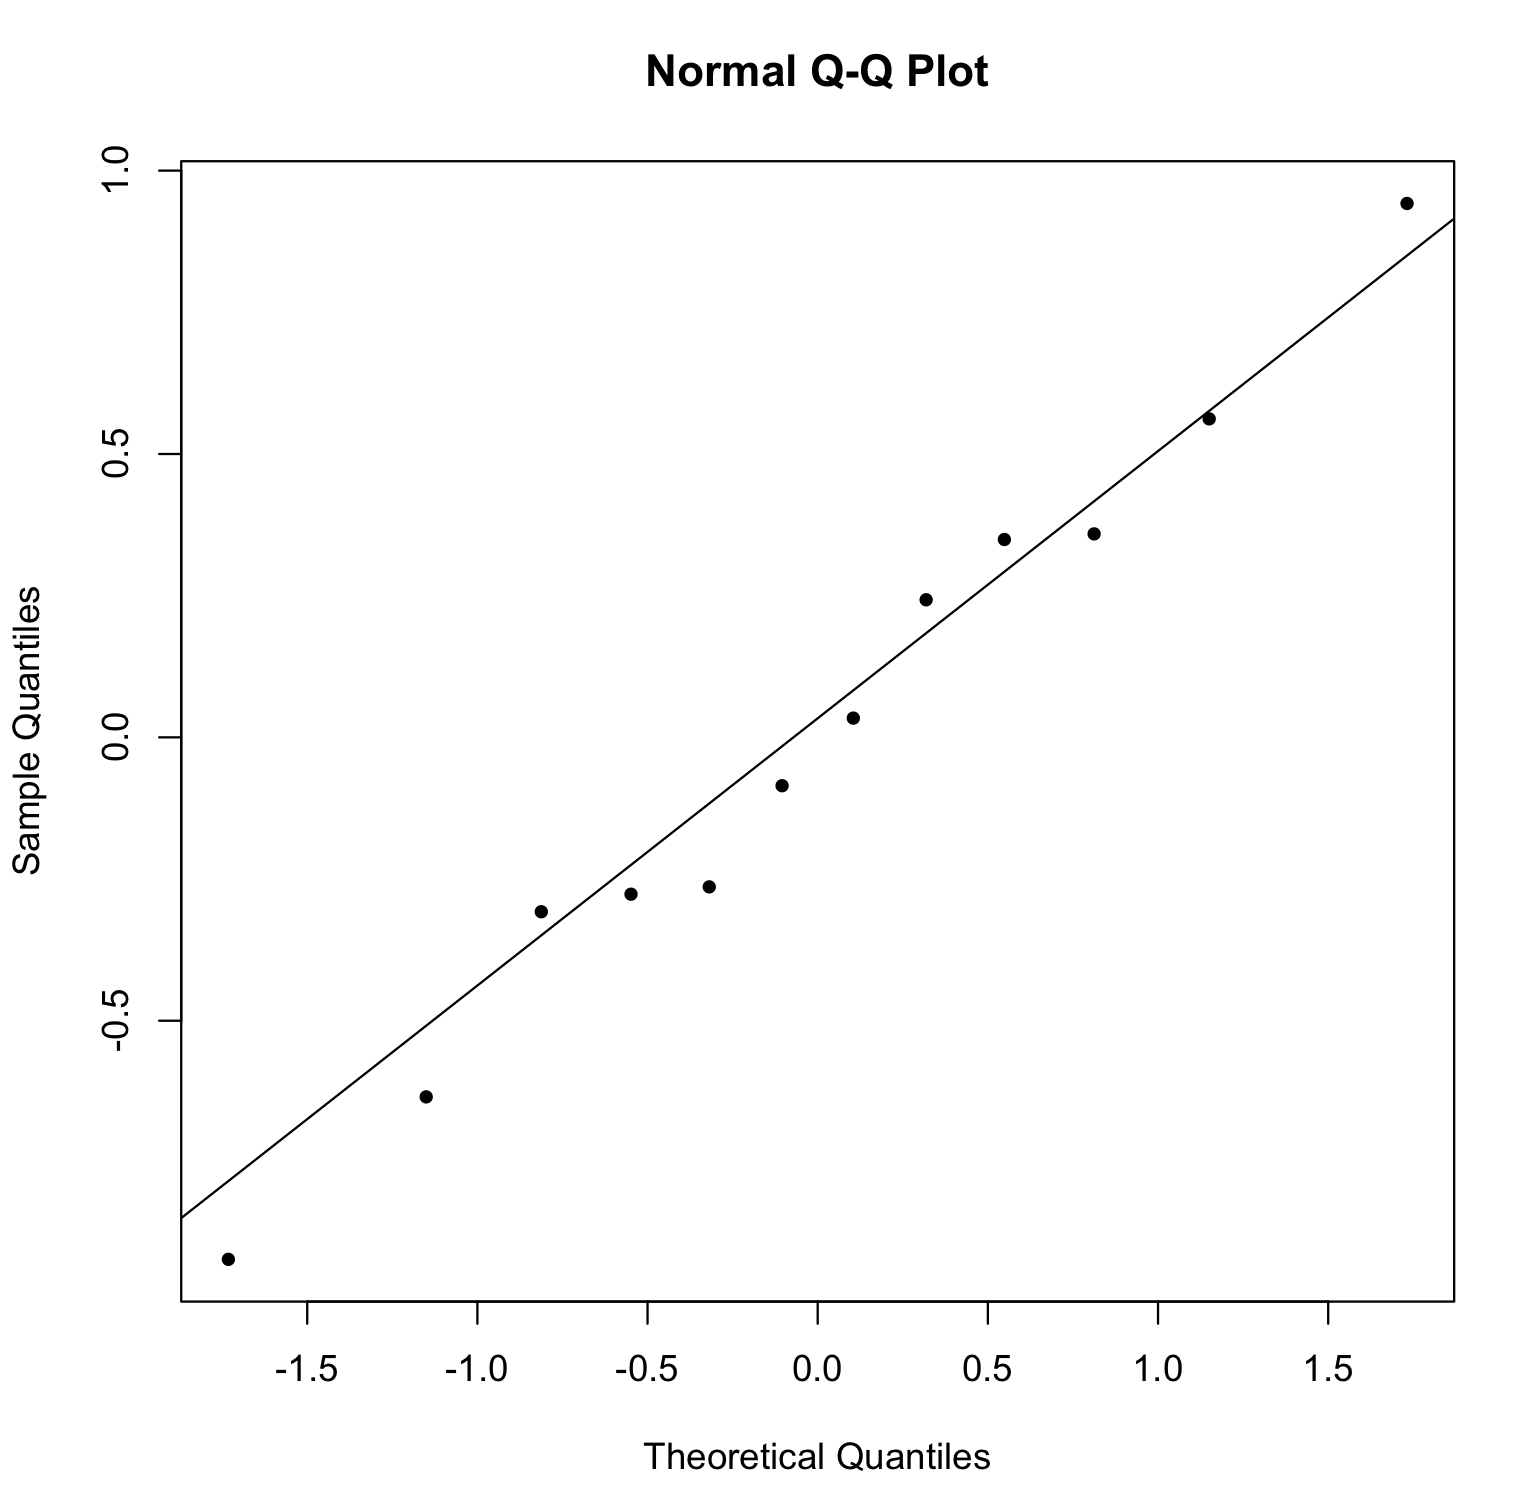
\includegraphics[width=\textwidth]{../pictures/hw3_q1_2_qq.png}
    \end{subfigure}
    \begin{subfigure}{0.45\textwidth}
        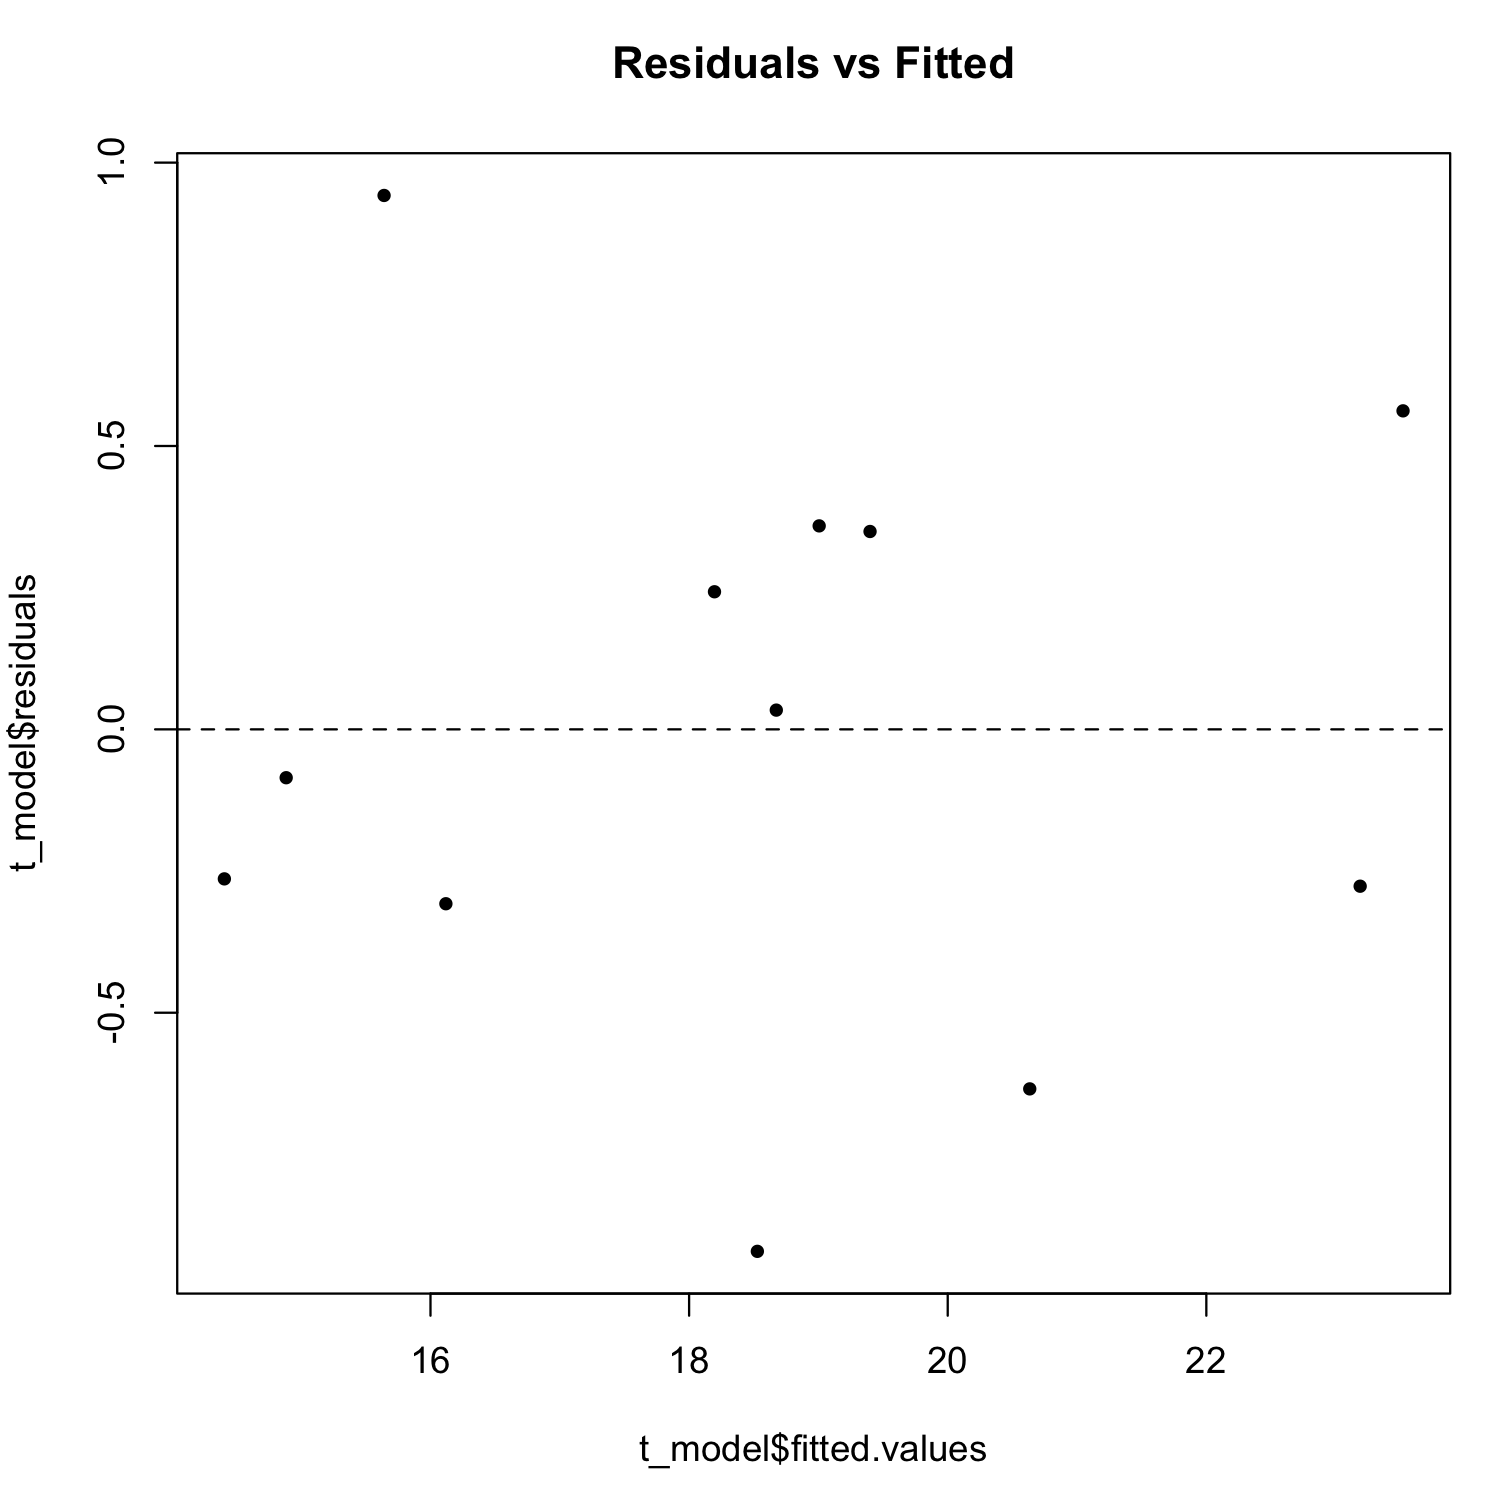
\includegraphics[width=\textwidth]{../pictures/hw3_q1_2_nf.png}
    \end{subfigure}
\end{figure}

There does not seem to be a problem with normality as the plots are generally in a straight line.
And the residuals are almost equally distributed around the 0 line without large outliers. Hence there is nothing too unusual about the residuals.

\clearpage
% % % % % % % % % % % % % % % % % % % % % % % % % % % % % % % % % % % % % % % 
% % % %                 Question 2                              % % % % % % % 
% % % % % % % % % % % % % % % % % % % % % % % % % % % % % % % % % % % % % % % 

\section{Question 2}

In this problem I need to compare $\displaystyle a=3$ treatments (oil), 
but the data is being influenced by $\displaystyle b=5$ blocks (truck).

Analyse the data using ANOVA table, which is generated using below R code

\begin{lstlisting}[language=R]

    fuel=c(0.500, 0.634, 0.487, 0.329, 0.512,
            0.535, 0.675, 0.520, 0.435, 0.540,
            0.513, 0.595, 0.488, 0.400, 0.510)
    oil = factor(kronecker(c(1:3), rep(1,5) ) )
    truck = factor(rep(1:5,3))
    options(contrasts=c("contr.treatment","contr.poly"))
    model1=lm(fuel~oil+truck)

    summary(aov(model1))
    
\end{lstlisting}

\lstinputlisting[float=h,frame=tb,caption=R output,label=zebra]{../out/hw3_q2_anova.txt}

The model F-value of 6.353 implies the model is significant.

\paragraph{}
Fisher LSD comparisons allow each pair of treatment means to be compared. 

If $\displaystyle \mid \bar{y_i} - \bar{y_j} \mid > LSD$ then the treatment means  $\displaystyle i$ and $\displaystyle j$ are significantly different. 

Determine the treatment means using below R code

\begin{lstlisting}[language=R]
    mean(fuel[oil == 1])
    mean(fuel[oil == 2])
    mean(fuel[oil == 3])
    
    library(agricolae)
    lsd <- LSD.test(model1,"fuel")
    lsd    
\end{lstlisting}

\lstinputlisting[float=h,frame=tb,caption=R output,label=zebra]{../out/hw3_q2_means.txt}

Thus we have the treatment means as,
$\displaystyle \mu_1=0.4924, \mu_2=0.541, \mu_3=0.5012$

Based on examination of the plot, we would conclude that 
$\displaystyle \mu_1$ and $\displaystyle \mu_3$ are the same.
$\displaystyle \mu_2$ differs from $\displaystyle \mu_1$ and $\displaystyle \mu_3$;

\subsection{Residual Analyses}

\begin{figure}[H]
    \centering
    \begin{subfigure}{0.45\textwidth}
        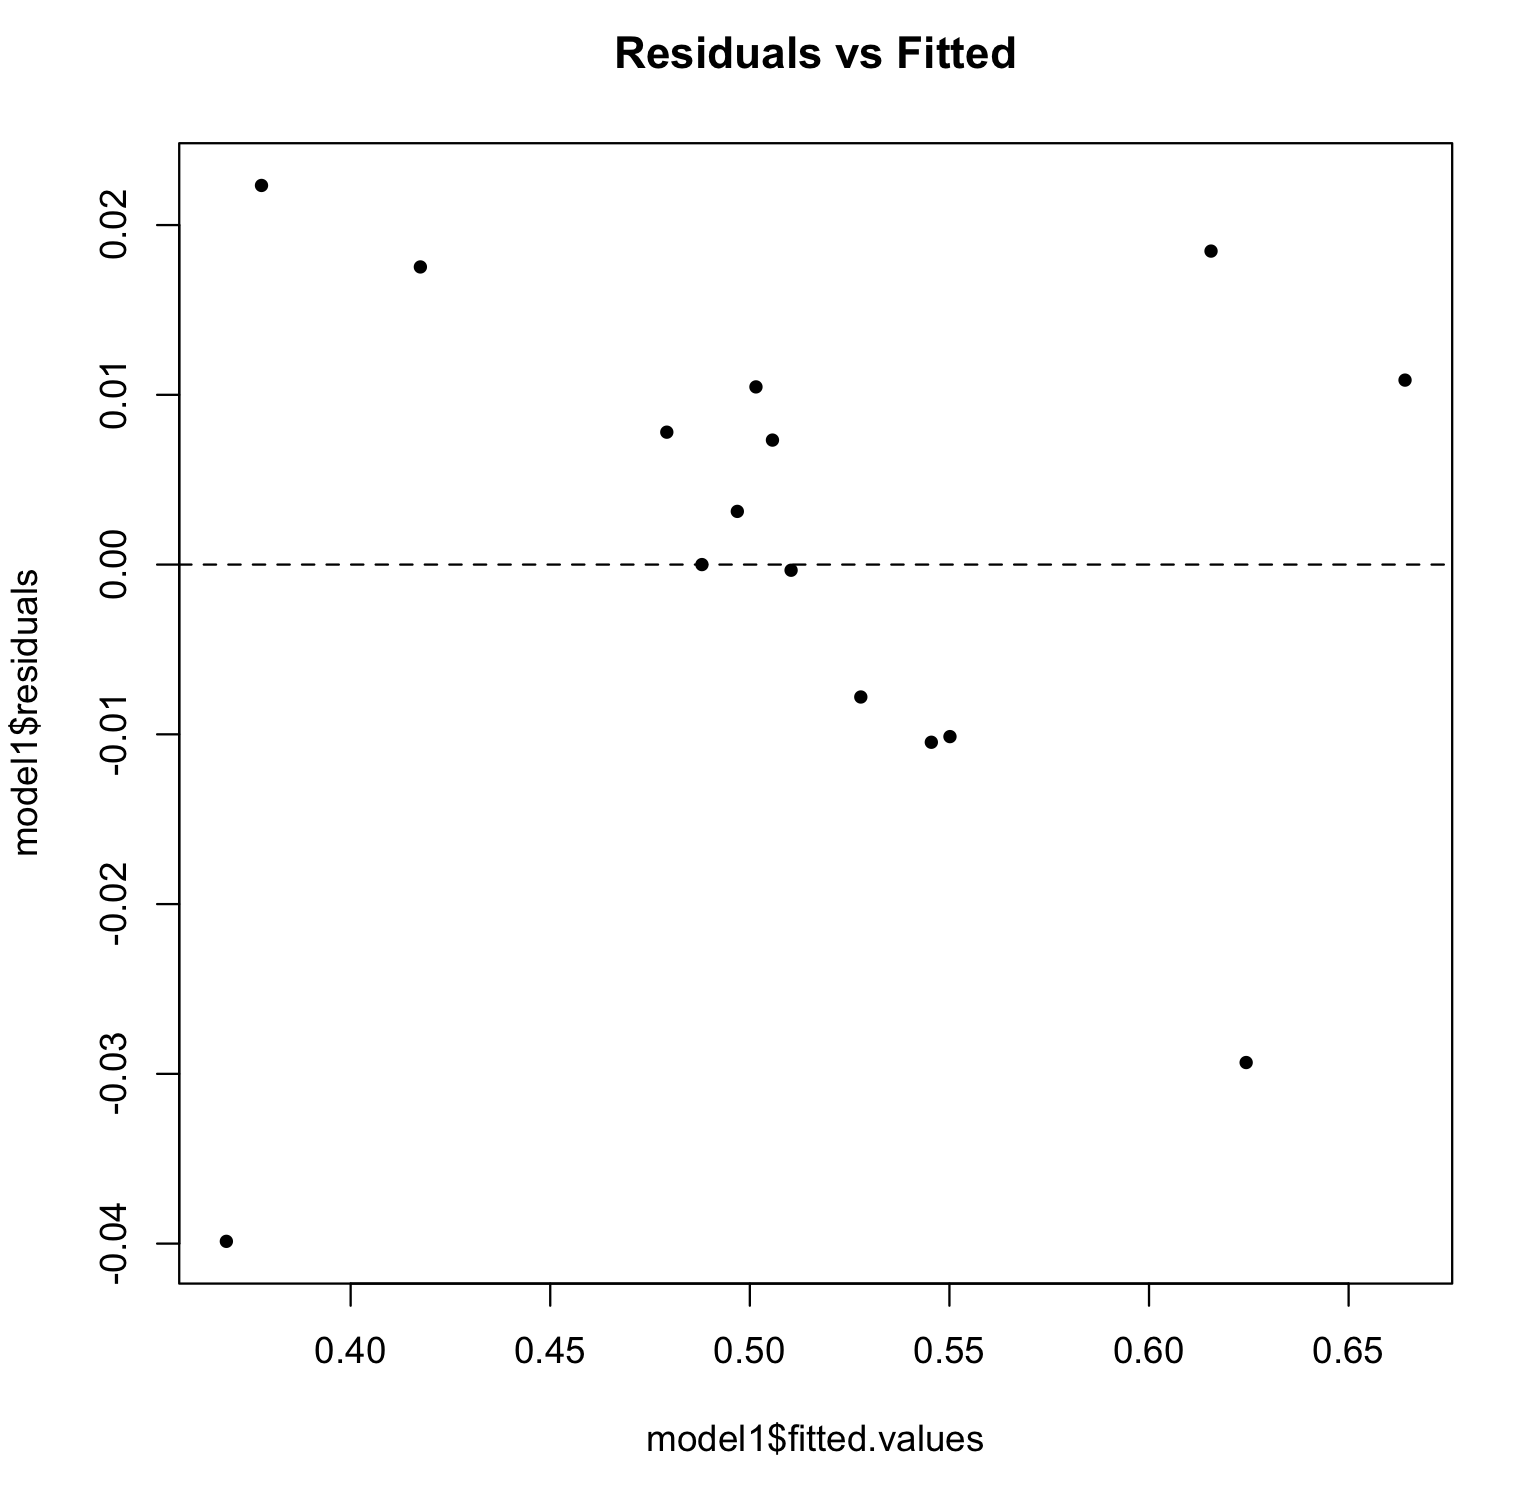
\includegraphics[width=\textwidth]{../pictures/hw3_q2_qq.png}
    \end{subfigure}
    \begin{subfigure}{0.45\textwidth}
        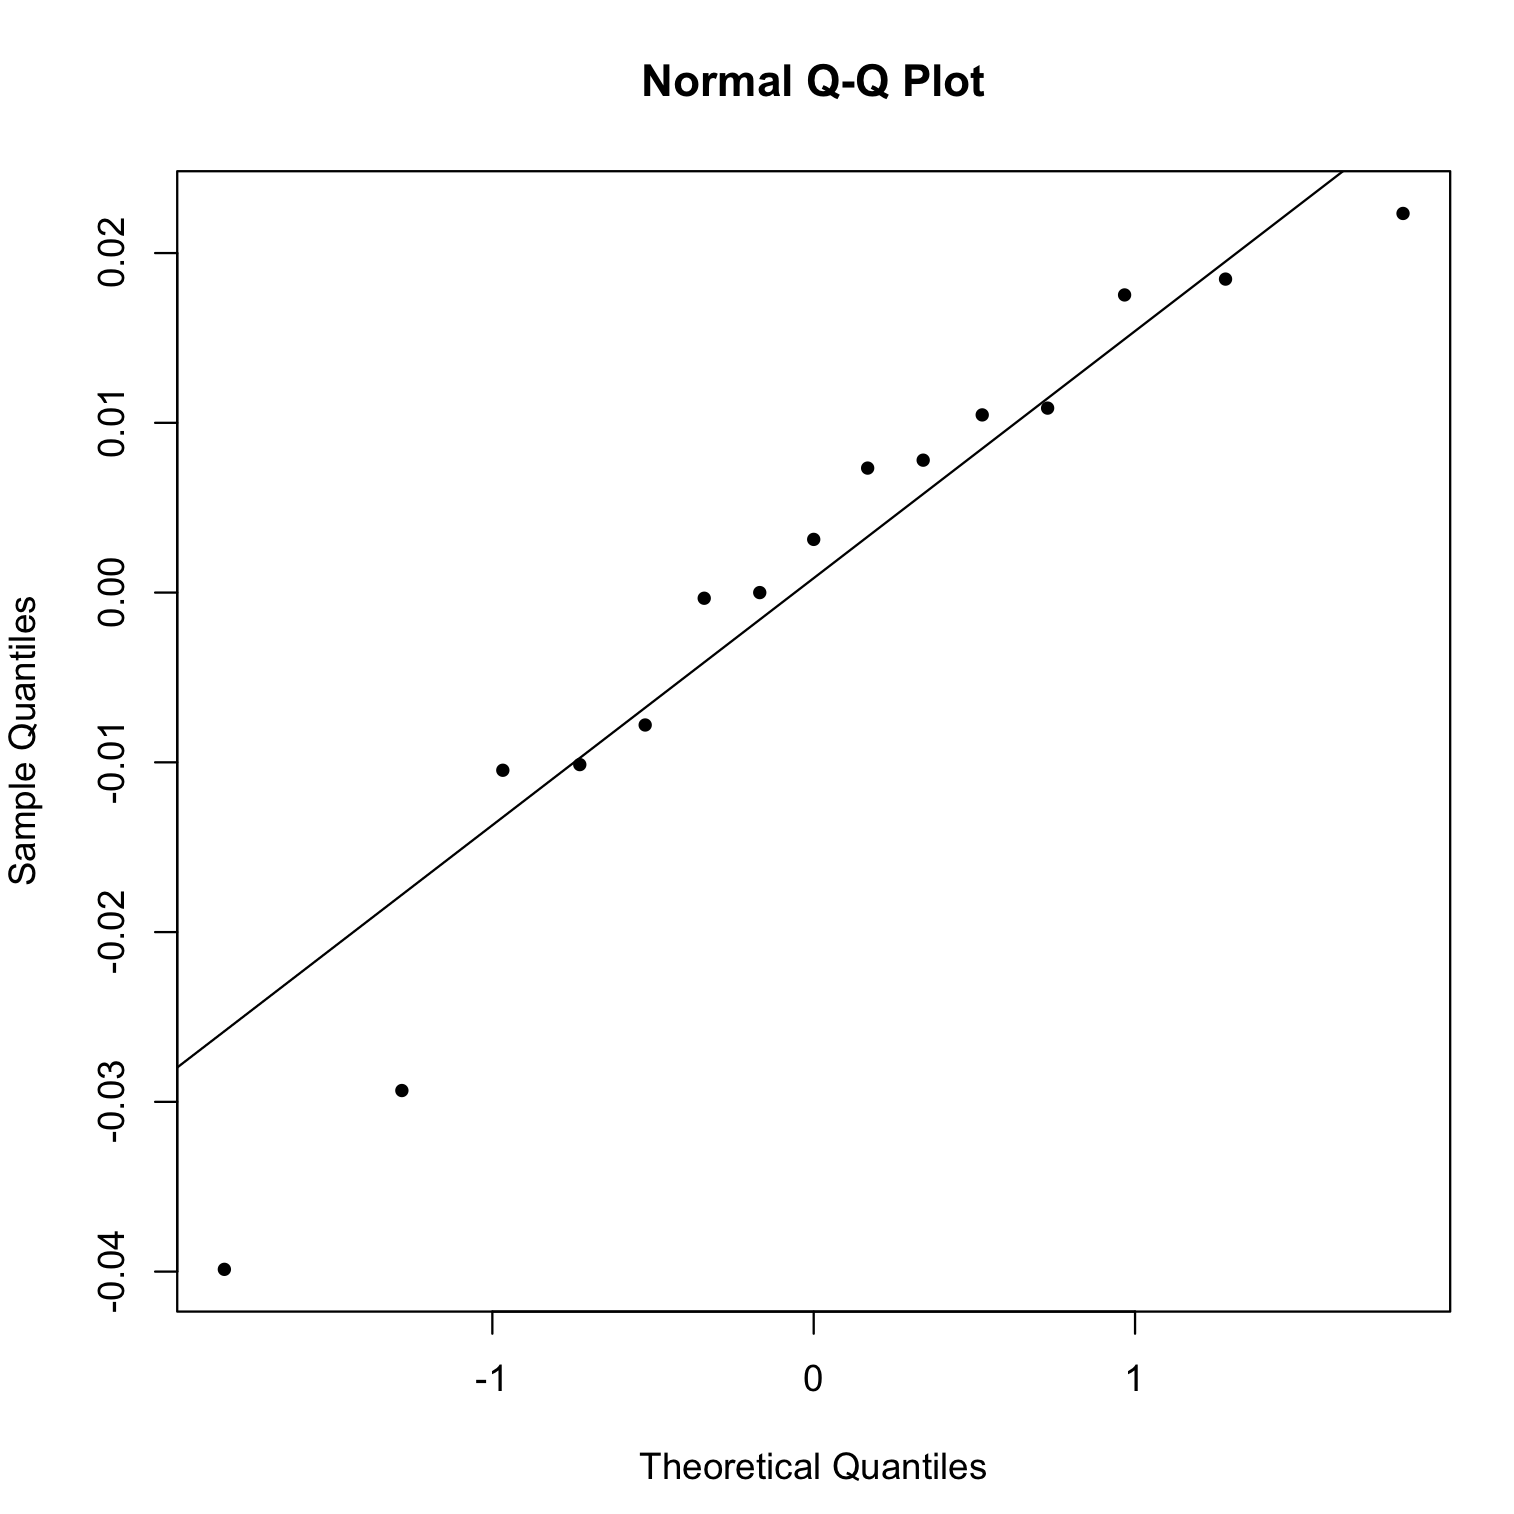
\includegraphics[width=\textwidth]{../pictures/hw3_q2_nf.png}
    \end{subfigure}
\end{figure}

There does not seem to be a problem with normality as the plots are generally in a straight line.
And the residuals are almost equally distributed around the 0 line without large outliers. Hence there is nothing too unusual about the residuals.

\end{document}
